% !TEX program = pdflatex
% 近代物理实验 A类超声诊断与超声特性综合实验
\documentclass[UTF8,10pt,a4paper]{article}
\usepackage{ctex}
% \catcode`\。=\active
% \newcommand{。}{.}
\newcommand{\CourseName}{近代物理实验}
\newcommand{\CourseCode}{PHYS1701}
\newcommand{\Semester}{2019-2020学年第学期}
\newcommand{\ProjectName}{A类超声诊断与超声特性综合实验}
\newcommand{\TimeType}{实验日期}
\newcommand{\Time}{2020. 5. 20(周三)}
\newcommand{\StudentName}{陈稼霖}
\newcommand{\StudentID}{45875852}
\usepackage[vmargin=1in,hmargin=.5in]{geometry}
\usepackage{fancyhdr}
\usepackage{lastpage}
\usepackage{calc}
\pagestyle{fancy}
\fancyhf{}
\fancyhead[L]{\CourseName}
\fancyhead[C]{\ProjectName}
\fancyhead[R]{\StudentName}
\fancyfoot[R]{\thepage\ / \pageref{LastPage}}
\setlength\headheight{12pt}
\fancypagestyle{FirstPageStyle}{
    \fancyhf{}
    \fancyhead[L]{\CourseName\\
        \CourseCode\\
        \Semester}
    \fancyhead[C]{{\huge\bfseries\ProjectName}\\
        \TimeType\ : \Time}
    \fancyhead[R]{姓名 : \makebox[\widthof{\StudentID}][s]{\StudentName}\\
        学号 : \StudentID\\
        成绩 : \underline{\makebox[\widthof{\StudentID}]{}}}
    \fancyfoot[R]{\thepage\ / \pageref{LastPage}}
    \setlength\headheight{36pt}
}
\usepackage{amsmath,amssymb,amsthm,bm}
\allowdisplaybreaks[4]
\usepackage{multirow}
\usepackage{graphicx}
\usepackage{subfigure}
\begin{document}
\thispagestyle{FirstPageStyle}
\section{准备工作}
在水箱中注入清水至没过超声波探头1cm左右,将探头与试验仪主机的“超声探头”接口相连,将主机的“信号输出”接口与示波器的CH1相连. 将示波器调至交流信号档,使用上升沿触发方式,并找到一适当的触发电平使波形稳定.

\section{测量水中超声波的传播速率}
将铝合金短圆柱样品固定在样品架上,将样品架搁在导轨上并微调角度使发射信号最大. 可以观察到一个不随样品架滑动而改变的、较强的信号峰,这是超声波从探头发出进入水中时的反射波,此外在其后方还有几个等间距分布的、会随样品架滑动而同步移动位置的信号峰,这些峰随着反射时间的推移而衰减,其中的第一个峰就是超声波被样品第一反射面反射而接收到的信号,后面的这些峰是超声波在样品前后放射面间被多次来回反射后接收到的信号.

以2cm的步长移动样品架,测出样品架在各个位置时超声探头与样品第一反射面间超声波的传播时间,所得数据如表\ref{2-T}所示.

\begin{table}[h]
    \centering
    \caption{水中超声波传播速率的测量数据}
    \label{2-T}
    \begin{tabular}{|c|c|c|c|c|c|c|c|c|c|c|}
        \hline
        样品架的位置 $X$ / cm & 2.00 & 4.00 & 6.00 & 8.00 & 10.00 & 12.00 & 14.00 & 16.00 & 18.00 & 20.00 \\ \hline
        \begin{tabular}[c]{@{}c@{}}超声探头与样品第一反射面间\\ 超声波的传播时间 $t$ / $\mu$s\end{tabular} & 15.10 & 41.40 & 67.80 & 94.40 & 121.2 & 148.4 & 176.0 & 202.8 & 228.8 & 255.6 \\ \hline
        传播时间的一半 ($t/2$) / $\mu$s & 7.55 & 20.70 & 33.90 & 47.20 & 60.60 & 74.20 & 88.00 & 101.4 & 114.4 & 127.8 \\ \hline
    \end{tabular}
\end{table}

做样品架的位置$X$关于传播时间的一半$(t/2)$的线性拟合,如图所示\ref{2-F},拟合线的斜率为$v=0.149\text{cm}/\mu\text{s}=1.49\times 10^3\text{m}/\text{s}$,这就是超声波在水中的传播速率.
\begin{figure}[h]
    \centering
    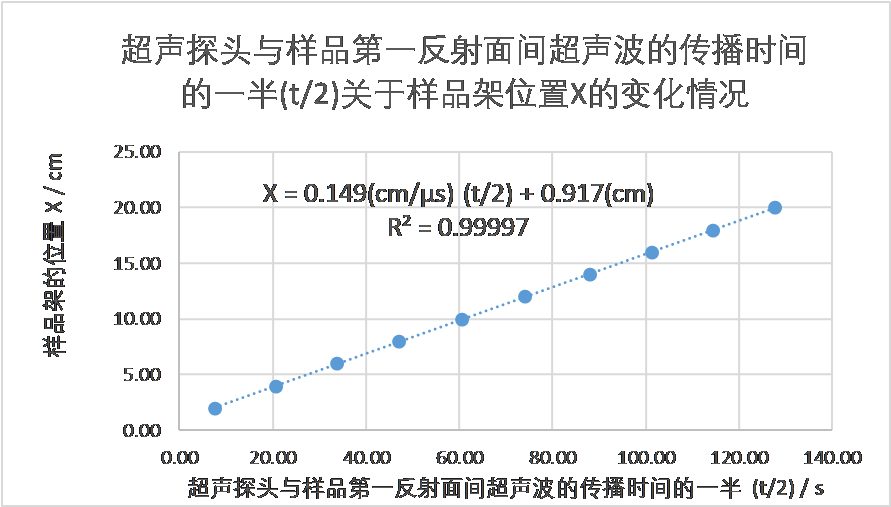
\includegraphics[width=.6\textwidth]{2-F.png}
    \caption{超声探头与样品第一反射面间超声波的传播时间的一般(t2)关于样品架位置X的变化情况.}
    \label{2-F}
\end{figure}

\section{测量样品中的超声波传播速率}
将圆柱样品分别固定在样品架上,将样品架搁在导轨上并微调样品架使反射信号最大. 测出样品架第一反射面的回波与第二反射面的回波的时间差的一半$\frac{t_2-t_1}{2}$(第一反射面的回波在示波器屏幕上对应第一个会随样品移动而移动的峰,第二反射面的回波在示波器屏幕上对应与前者同步随样品移动而移动、相对时间差保持不变的峰,我们利用了示波器的辅助线功能直接读出这两个峰的时间差),量出样品长度$d$(注意,对于较短的样品我们使用精度更高的螺旋测微仪进行测量,对于长度超出螺旋测微仪量程的样品我们使用量程更大的游标卡尺进行测量,当使用螺旋测微仪进行测量时,应当从读数中减去零误差,当使用游标卡尺进行测量时,因为有些样品的圆柱有凸出来的圆环部分,所以先测量总长,再减去这一突出来的圆环部分的长度),算出超声波在样品中的传播速率$\frac{2d}{t_2-t_1}$. 三种材料六个圆柱样品的测量和计算结果如表\ref{3-T}.
\begin{table}[h]
    \centering
    \footnotesize
    \caption{圆柱体样品中超声波的传播速率的测量数据记录表}
    \label{3-T}
    \begin{tabular}{|c|c|c|c|c|c|c|c|c|c|c|c|}
    \hline
    \multirow{3}{*}{样品种类} & \multicolumn{6}{c|}{\begin{tabular}[c]{@{}c@{}}样品第一反射面回波和第二反射面回波时间差\\ $t_1-t_2$ / $\mu$s\end{tabular}} & \multirow{3}{*}{\begin{tabular}[c]{@{}c@{}}回波时间差\\ 的一半\\ $\frac{t_2-t_1}{2}$ / $\mu$s\end{tabular}} & \multirow{3}{*}{\begin{tabular}[c]{@{}c@{}}螺旋测微仪/\\ 游标卡尺读数\\ / mm\end{tabular}} & \multirow{3}{*}{\begin{tabular}[c]{@{}c@{}}螺旋测微仪零误差/\\ 凸出来的圆环部分\\ 的长度 / mm\end{tabular}} & \multirow{3}{*}{\begin{tabular}[c]{@{}c@{}}样品长度\\ $d$ / mm\end{tabular}} & \multirow{3}{*}{\begin{tabular}[c]{@{}c@{}}超声波在样品中\\ 的传播速率 $v$\\ / m$\cdot$s$^{-1}$\end{tabular}} \\ \cline{2-7}
     & \multicolumn{5}{c|}{测量次数} & \multirow{2}{*}{平均值} &  &  &  &  &  \\ \cline{2-6}
     & 1 & 2 & 3 & 4 & 5 &  &  &  &  &  &  \\ \hline
    \begin{tabular}[c]{@{}c@{}}铝合金\\ 短圆柱\end{tabular} & 8.20 & 8.20 & 8.20 & 8.10 & 8.00 & 8.14 & 4.07 & 25.008 & -0.006 & 25.014 & 6.15E+03 \\ \hline
    \begin{tabular}[c]{@{}c@{}}铝合金\\ 长圆柱\end{tabular} & 16.00 & 16.00 & 16.20 & 16.40 & 16.20 & 16.16 & 8.08 & 52.08 & 2.00 & 50.08 & 6.198E+03 \\ \hline
    \begin{tabular}[c]{@{}c@{}}冕玻璃\\ 短圆柱\end{tabular} & 9.00 & 9.00 & 9.00 & 9.00 & 9.00 & 9.00 & 4.50 & 24.958 & -0.006 & 24.964 & 5.55E+03 \\ \hline
    \begin{tabular}[c]{@{}c@{}}冕玻璃\\ 长圆柱\end{tabular} & 18.40 & 18.00 & 18.00 & 18.00 & 18.20 & 18.12 & 9.06 & 50.56 & 0.56 & 50.00 & 5.519E+03 \\ \hline
    \begin{tabular}[c]{@{}c@{}}有机玻璃\\ 短圆柱\end{tabular} & 5.52 & 5.64 & 5.56 & 5.56 & 5.56 & 5.57 & 2.78 & 7.500 & \multirow{2}{*}{-0.006} & 7.506 & 2.70E+03 \\ \cline{1-9} \cline{11-12} 
    \begin{tabular}[c]{@{}c@{}}有机玻璃\\ 长圆柱\end{tabular} & 11.30 & 11.30 & 11.30 & 11.30 & 11.30 & 11.30 & 5.65 & 15.124 &  & 15.124 & 2.677E+03 \\ \hline
    \end{tabular}
\end{table}

综合各种材料长短圆柱样品的超声波传播速率(取平均值)
\begin{itemize}
    \item $u_{\text{铝合金}}=6.17\times 10^3$m/s.
    \item $u_{\text{冕玻璃}}=5.53\times 10^3$m/s.
    \item $u_{\text{有机玻璃}}=2.69\times 10^3$m/s.
\end{itemize}

\section{模拟人体脏器超声定位诊断}
选用样品1为冕玻璃短圆柱,样品2为铝合金短圆柱. 如图\ref{4},使样品1与探头相隔一小段距离(样品架1在滑轨上的坐标为$5.00$cm),作为腹壁,样品2与样品1相隔一定距离(样品架2在滑轨上的坐标为$15.00$cm),作为内脏,从而模拟超声波定位诊断测量环境. 测量前要尝试移动两个样品,根据示波器屏幕上峰的移动情况鉴别各个反射面的信号.

\begin{figure}[h]
    \centering
    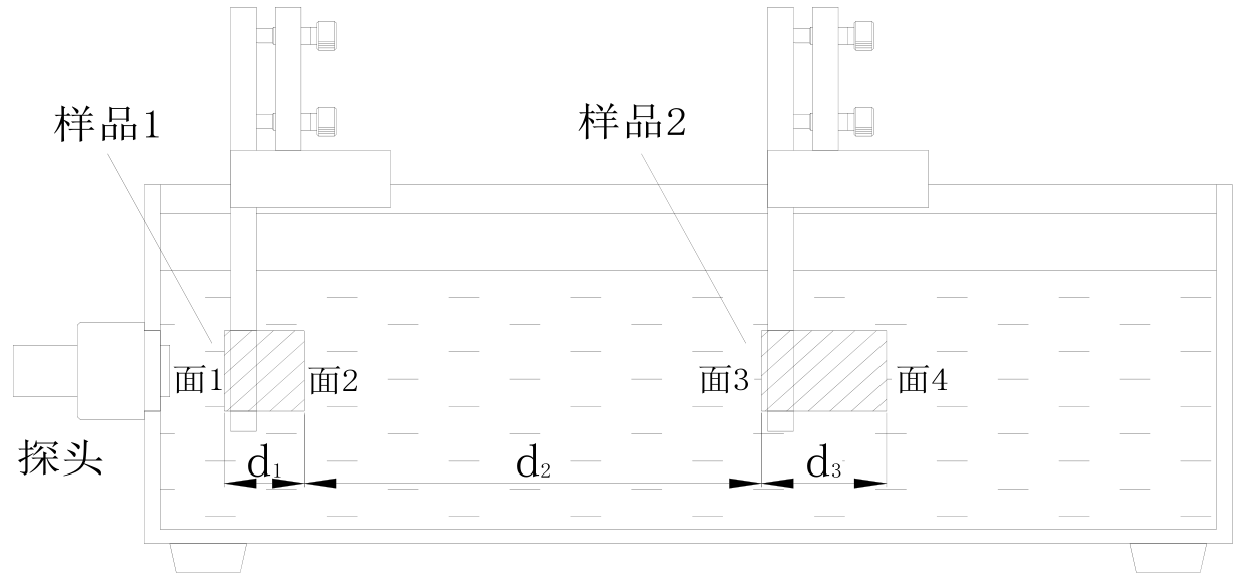
\includegraphics[width=.6\textwidth]{4.png}
    \caption{超声定位诊断模拟实验的装置图.}
    \label{4}
\end{figure}

在测量过程中,发现第二个样品的反射信号相对第一个样品衰减了很多,这说明如果真正要将超声波应用于人体脏器诊断,其功率要比本次式样所用仪器($10\text{mW}/\text{cm}^2$)高出很多.

测量结果:
\begin{enumerate}
    \item 样品1的第一个反射面回波和样品1的第二个反射面回波时间差为$t_2-t_1=8.80\mu$s.
    \item 样品1的第一个反射面回波和样品2的第一个反射面回波时间差为$t_3-t_1=111.2\mu$s.
    \item 样品1的第一个反射面回波和样品2的第二个反射面回波时间差为$t_4-t_1=120.4\mu$s.
\end{enumerate}

计算结果:
\begin{enumerate}
    \item 腹腔的厚度为$d_1=u_{\text{冕玻璃}}\frac{t_2-t_1}{2}=5.53\times\frac{8.80}{2}\text{mm}=24.3$mm,与其实际长度$24.964$mm的相对误差为$-2.48\%$,符合得较好.
    \item 腹腔到脏器表面的距离为$v\frac{t_3-t_2}{2}=v\frac{(t_3-t_1)-(t_2-t_1)}{2}=1.49\times\frac{111.2-8.80}{2}\text{mm}=76.3$mm,实际上,两个样品架相距$10.00$cm(虽然不准确,但是可以作为两个样品的第一反射面间的距离的参考),样品1的长度为$24.964$mm,故样品1的第二反射面到样品2的第一反射面的实际距离约为$75.04$mm,可见超声波探测得到的长度与实际长度符合得较好.
    \item 脏器厚度为$u_{\text{铝合金}}\frac{(t_4-t_3)}{2}=u_{\text{铝合金}}\frac{(t_4-t_1)-(t_3-t_1)}{2}=6.17\times\frac{120.4-111.2}{2}\text{mm}=28.4$mm,与其实际长度$25.014$mm的相对误差为$13.5\%$,可见信号衰减后测得的长度误差变大.
\end{enumerate}

\section{分辨力测量实验}
将分辨力样块通过两个手拧螺丝固定在横向滑块的底部,搁置在横向导轨的中间位置,使超声探头能够通过样块前表面探测到后表面中间台阶左右不同声程的信号. 如图\ref{5},当两个信号的间距小于峰宽$b$时,这两个信号的峰就会重叠在一起而无法被分辨出,因此峰宽$b$对应的长度即为超声波的所能分辨的最小长度,即超声波的分辨力.

\begin{figure}[h]
    \centering
    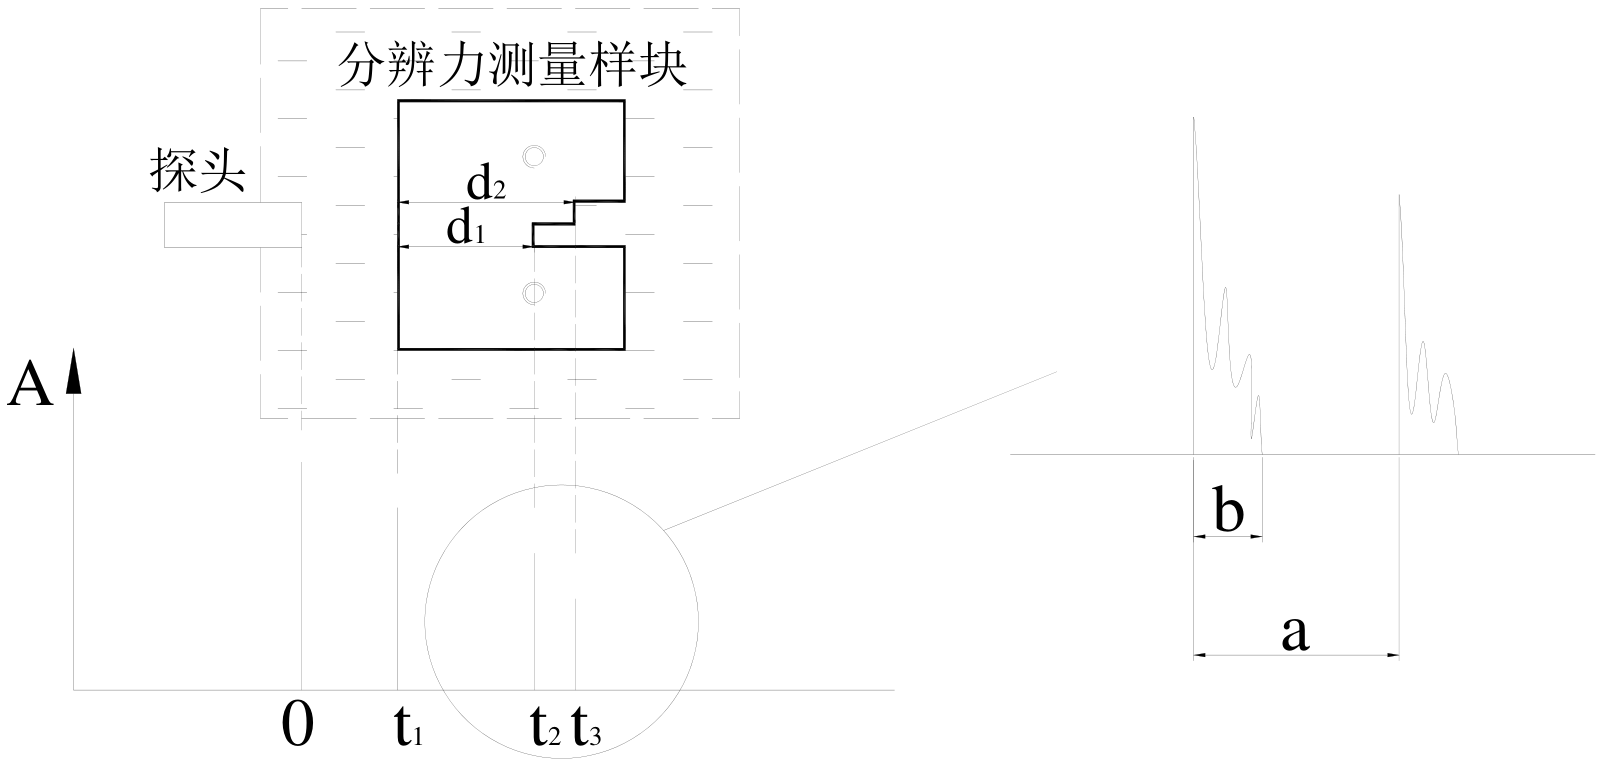
\includegraphics[width=.6\textwidth]{5.png}
    \caption{测量超声实验仪对铝合金材料的分辨力实验示意图.}
    \label{5}
\end{figure}

我们测量出样块前表面到中间第一个台阶的距离为$d_1=29.62$mm,样块前表面到中间第二个台阶的距离为$d_2=39.16$mm,中间第一个台阶反射波的峰宽为$b=4.95\mu$s,第一个台阶反射波和第二个台阶反射波的时间差为$a=12.56\mu$s,故超声波的分辨力为
\begin{align}
    F=(d_2-d_1)\frac{b}{a}=(39.16-29.62)\times\frac{4.95}{12.56}\text{mm}=3.76\text{mm}.
\end{align}

\section{超声脉冲反射法探伤}
将有不同深度的两条细缝的铝合金工件样块(如图\ref{6-2})固定在横向滑块的底部(如图\ref{6-1}),搁置在横向导轨的中间位置. 将横向滑块左右滑动,观察示波器屏幕上各个信号峰的涨落,从而可以分辨出各个信号峰所对应的反射面.

\begin{figure}[h]
	\centering
	\subfigure[铝合金工件样块.]{
	\label{6-2}
	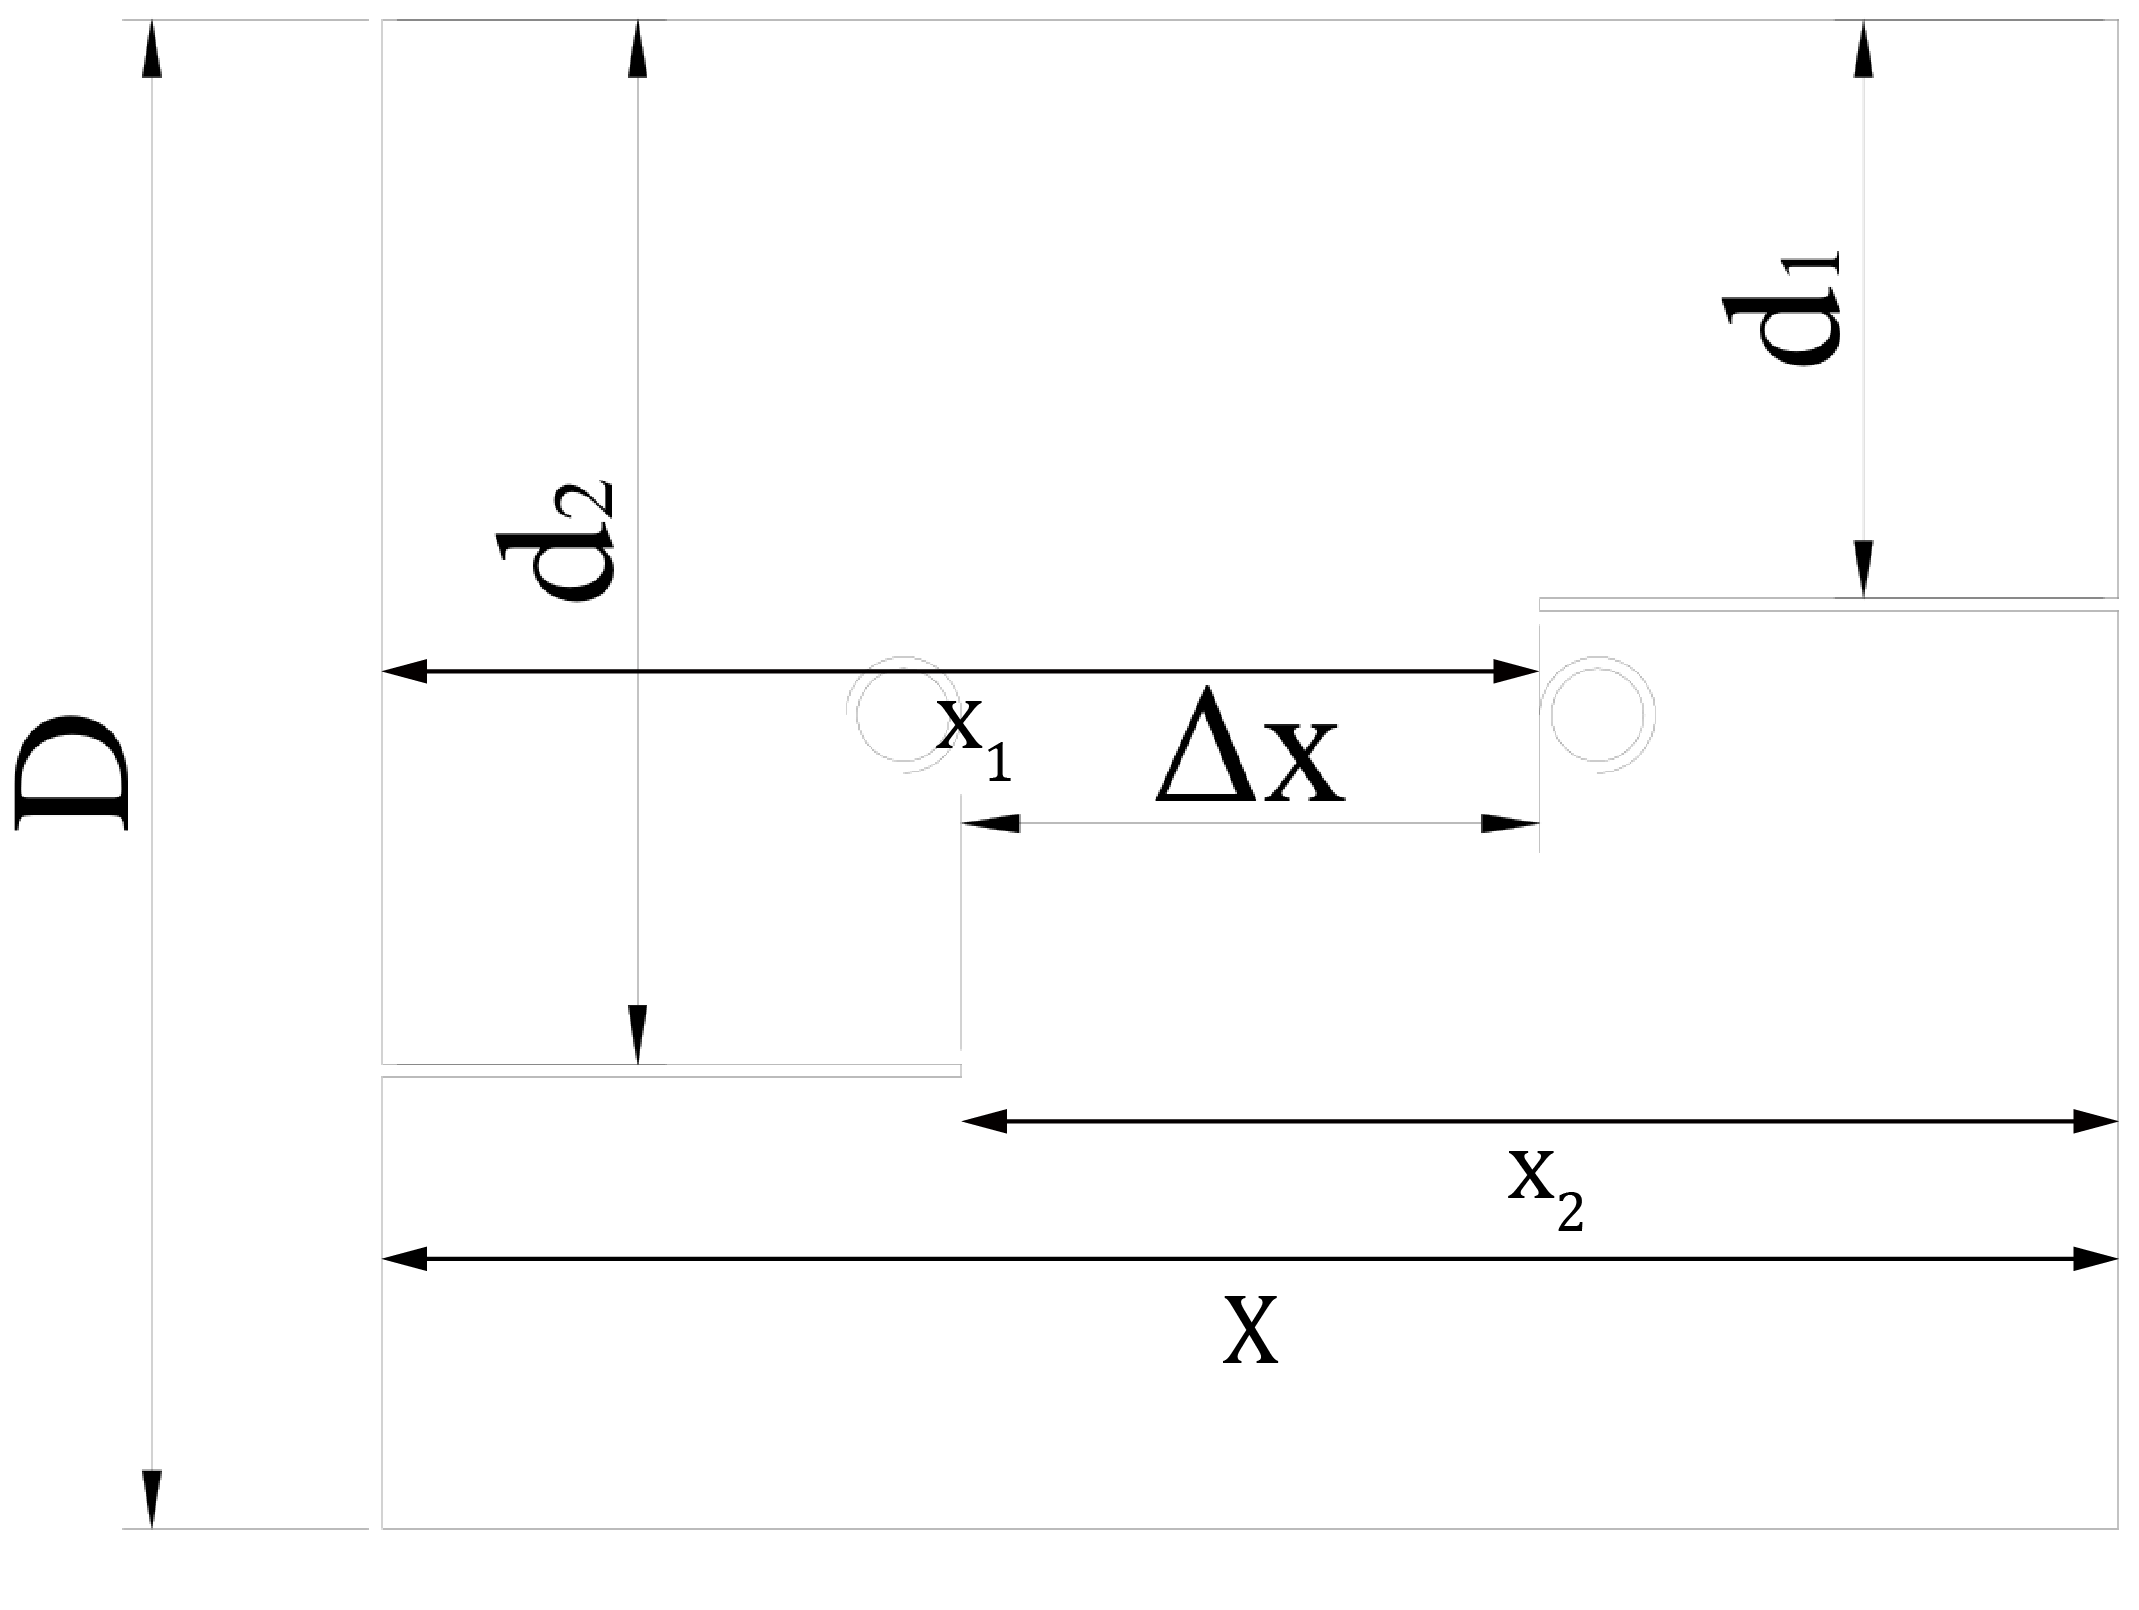
\includegraphics[width=0.45\textwidth]{6-2(1).png}}
	\subfigure[超声脉冲反射法探伤实验装置图.]{
	\label{6-1}
	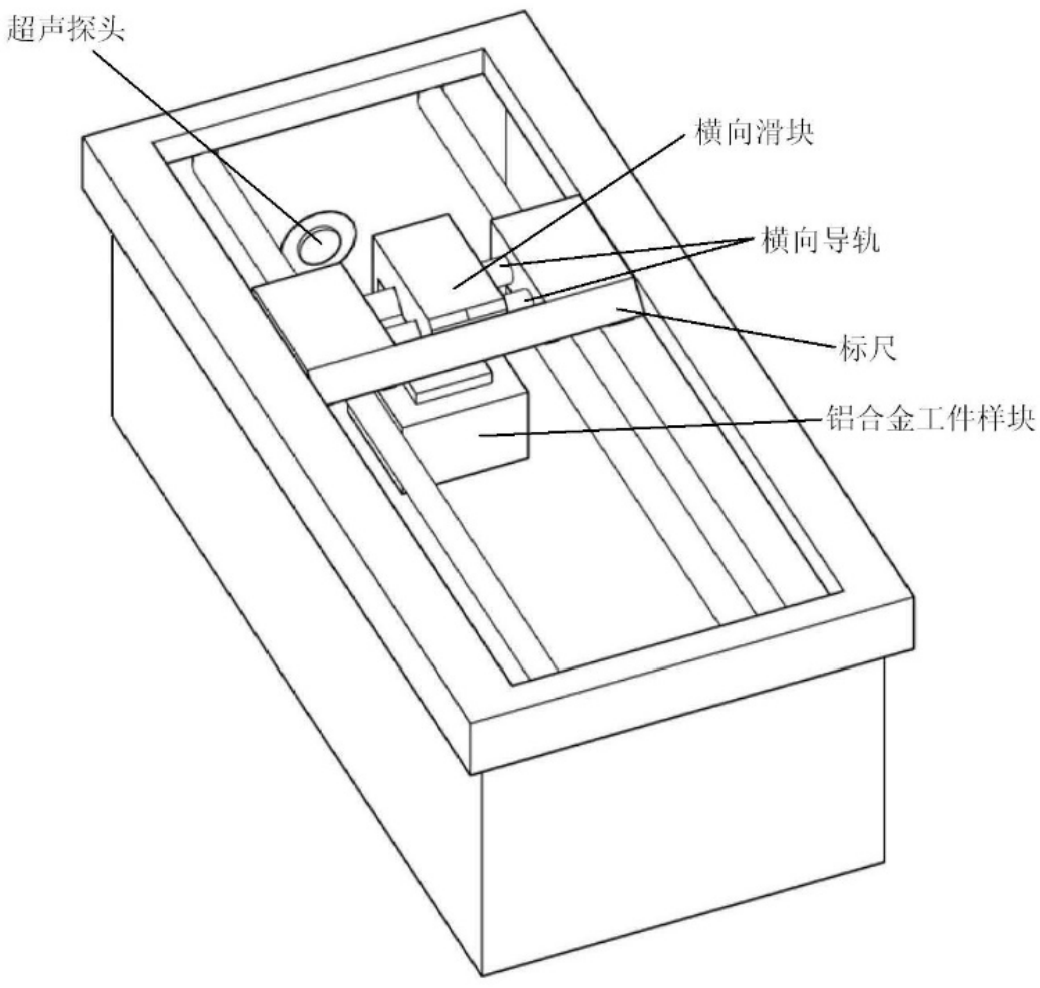
\includegraphics[width=0.45\textwidth]{6-1.png}}
\end{figure}

我们测量出工件样块前表面反射波与第一条细缝反射波的时间差为$t_2-t_1=8.00\mu$s,工件样块前表面反射波与第二条细缝反射波的时间差为$t_3-t_1=14.40\mu$s,工件样块前表面反射波与后表面反射波的时间差为$t_4-t_1=20.80\mu$s,工件样块前表面到后表面的距离为$D=64.84$mm,故计算得工件样块前表面到第一条细缝的距离为
\begin{align}
    d_1=\frac{t_2-t_1}{t_4-t_1}D=\frac{8.00}{20.80}\times 64.84\text{mm}=24.9\text{mm}.
\end{align}
实际测量得工件样块前表面到第一条细缝的距离为$24.72$mm,故超声探测的相对误差为$0.883\%$,符合得很好. 计算的工件样块后表面到第二条细缝的距离为
\begin{align}
    d_2=\frac{t_3-t_1}{t_4-t_1}D=\frac{14.40}{20.80}\times 64.84\text{mm}=44.89\text{mm}.
\end{align}
实际测量得工件样块前表面到第二条细缝的距离为$45.06$mm,故超声探测的相对误差为$-0.379\%$,符合得很好.

左右移动横向滑块,分别读出第一条细缝反射信号和工件样块后表面反射信号达到相等时横向滑块在横向导轨上的位置坐标,以及第二条细缝反射信号和工件样块后表面反射信号达到相等时横向滑块在横向导轨上的位置坐标,两者之差为$8.08-5.82\text{cm}=2.26$cm,这就是两条细缝的横向间距$\Delta x$. 我们还实际测量了$x_1=49.96$mm,$x_2=50.04$mm,整个工件样块的横向宽度为$X=7.514$mm,故两条细缝的横向间距实际值为$x_1+x_2-X=(49.96+50.04-75.14)\text{mm}=24.86$mm,故超声探测的相对误差为$-9.09\%$,可见超声探伤的横向测量精度不及纵向测量精度.
\end{document}